\documentclass[french]{article}

\usepackage{amsmath} % for \text
\usepackage{amssymb} % for \mathbb
\usepackage{amsthm} % for proof environment
\usepackage{hyperref} % for \autoref
\usepackage{cleveref} % for \cref
\usepackage{tikz} % for tikzpicture
\usepackage{graphicx} % for \includegraphics
\usepackage{subcaption} % for subfigure
\usepackage{float} % for H in figure
\usepackage{geometry} % for \newgeometry
\usepackage{fullpage} % for fullpage
\usepackage{babel} % for french
\usepackage[T1]{fontenc} % for french
\usepackage{minted} % for code
\usepackage{xcolor} % to access the named colour LightGray
%New colors defined below
\definecolor{codegreen}{rgb}{0,0.6,0}
\definecolor{codegray}{rgb}{0.5,0.5,0.5}
\definecolor{codepurple}{rgb}{0.58,0,0.82}
\definecolor{backcolour}{rgb}{0.97,0.97,0.95}

\usepackage{listings}
\lstdefinestyle{mystyle}{
  language=python,
  backgroundcolor=\color{backcolour}, 
  commentstyle=\color{olive},
  keywordstyle=\color{violet},
  numberstyle=\tiny\color{codegray},
  stringstyle=\color{orange},
  basicstyle=\ttfamily\footnotesize,
  breakatwhitespace=false,         
  breaklines=true,                 
  captionpos=b,                    
  keepspaces=true,                               
  showspaces=false,                
  showstringspaces=false,
  showtabs=false,                  
  tabsize=2
}
\lstset{style=mystyle}


\definecolor{LightGray}{gray}{0.9}

\usepackage[backend=biber,style=numeric]{biblatex}

\addbibresource{references.bib}

\geometry{left = 1.8cm, right = 1.8cm}

\begin{document}

\begin{center}
    \textbf{\LARGE{Ecole Normale Supérieure de Paris-Saclay}}\\
\end{center}

\vspace{1cm}

\begin{center}
    \textbf{Rapport TER}
\end{center}

\noindent\rule{\textwidth}{0.6mm}
\bigskip
\begin{center}
    \textbf{\LARGE{TER - Voiture autonomes avec apprentissage par renforcement et lidar}}
\end{center}
\bigskip
\noindent\rule{\textwidth}{0.6mm}

\begin{center}
    \today
\end{center}

\bigskip
\begin{center}
    \textsc{Miquel Hugo}
\end{center}
\begin{center}
    \textsc{Plus Basile}
\end{center}

\begin{figure}[b]
    \centering
    \begin{minipage}[h]{0.45\textwidth}
        \raggedright
        
\includegraphics[width=0.6\textwidth]{Images/Logo-ENS-Paris-Saclay.png}
    \end{minipage}
    \begin{minipage}[h]{0.45\textwidth}
        \raggedleft
        
\includegraphics[width=0.6\textwidth]{Images/Logo-Universite-Paris-Saclay.jpg}
    \end{minipage}
\end{figure}


\newpage

\tableofcontents

\newpage

\section{Introduction}

\subsection{Contexte}

Les voitures autonomes sont un sujet de recherche très actif depuis quelques années. 
En effet, elles pourraient révolutionner le monde des transports en permettant de réduire les accidents de la route, 
de diminuer la consommation d'énergie et de réduire les embouteillages. 
Cependant, il reste encore de nombreux défis à relever pour que les voitures autonomes soient utilisées à grande échelle.
En particulier, il est nécessaire de développer des algorithmes d'apprentissage par renforcement qui permettent à une 
voiture autonome d'apprendre à conduire de manière autonome.

\subsection{Objectif et travail réalisé}
L'objectif de ce TER est de développer un algorithme d'apprentissage par renforcement qui permet à une 
voiture RC au format $1/10^{\text{ème}}$ de conduire de manière autonome sur un circuit. Dans un premier temps, nous 
avons utilisé Webots pour la simulation, gym et stable baselines pour l'apprentissage par renforcement.
Dans un second temps, nous avons transféré le réseau de neurones du simulateur à la voiture réelle.
La voiture est équipée d'un lidar qui permet de mesurer la distance entre la voiture et les murs du circuit.


\subsection{L'apprentissage par renforcement}
L'apprentissage par renforcement est une méthode d'apprentissage automatique qui permet à un agent 
d'apprendre à prendre des décisions en interagissant avec un environnement. 

\begin{figure}[H]
    \centering
    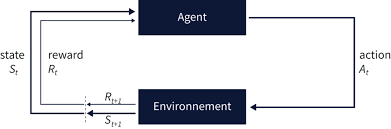
\includegraphics[width=0.6\textwidth]{Images/RL.png}
    \caption{Schéma de l'apprentissage par renforcement}
\end{figure}

L'agent prend des actions dans l'environnement et reçoit une récompense en fonction de l'action qu'il a prise. 
L'objectif de l'agent est de maximiser la somme des récompenses qu'il reçoit au cours des itérations.

\vspace{0.5cm}
Lors de chaque étape, l'agent reçoit une observation de l'environnement dans lequel il évolue. Sur la base 
de cette observation, l'agent prend une décision parmi un ensemble d'actions possible appelé espace des actions. 
Cet espace peut dépendre de l'état dans lequel se trouve l'agent.

\vspace{0.5cm}
Un exemple simple est celui d'un jeu d'échecs dans lequel l'observation correspond à la position de chacune des 
pièces sur l'échiquier et l'espace des actions est l'ensemble des déplacements possibles des pièces. 
Naturellement, on souhaite que l'agent réalise la meilleure action possible suivant l'observation reçue. 
Pour atteindre ce but, l'agent applique une politique d'action (notée $\pi$) qu'il utilise pour sa prise de décision.
À chaque récompense obtenue, cette politique est mise à jour. On espère ainsi atteindre une politique optimale.

\vspace{0.5cm}
Pour entraîner un agent, plusieurs types de méthodes peuvent être utilisées. Ces méthodes estiment la somme des 
récompenses futures que l'agent devrait obtenir. Ces récompenses sont pondérées pour favoriser les récompenses 
à court terme. La politique obtenue est souvent modélisée par un réseau de neurones, dont l'actualisation modifie 
les poids du réseau.

\vspace{0.5cm}
\noindent
Les méthodes d'apprentissage par renforcement peuvent être classées en trois catégories principales :
\begin{itemize}
\item \textbf{Méthodes basées sur la valeur (value-based)} : Ces méthodes se concentrent sur l'estimation de la récompense cumulative optimale que l'agent peut obtenir. Elles cherchent à obtenir une récompense cumulative maximale.
\item \textbf{Méthodes basées sur la politique (policy-based)} : Ces méthodes se concentrent sur l'optimisation de la politique de l'agent. Les valeurs de récompense peuvent ne pas être calculées directement.
\item \textbf{Méthodes acteur-critique (actor-critic)} : Ces méthodes utilisent deux réseaux de neurones. Le premier réseau choisit l'action à effectuer, tandis que le second réseau évalue cette action en la comparant à l'action prévue.
\end{itemize}


\section{Simulation}

\subsection{Le simulateur Webots}
Le logiciel utilisé pour la simulation est Webots R2023b. Webots est un logiciel de simulation de robotique développé 
par Cyberbotics. Il permet de simuler des robots dans un environnement 3D que l'on peut personnaliser. Dans notre cas,
nous avons utilisé Webots pour simuler une voiture RC sur un circuit. Nous avons utilisé le langage de programmation
Python pour contrôler la voiture dans le simulateur.

\begin{figure}[H]
    \centering
    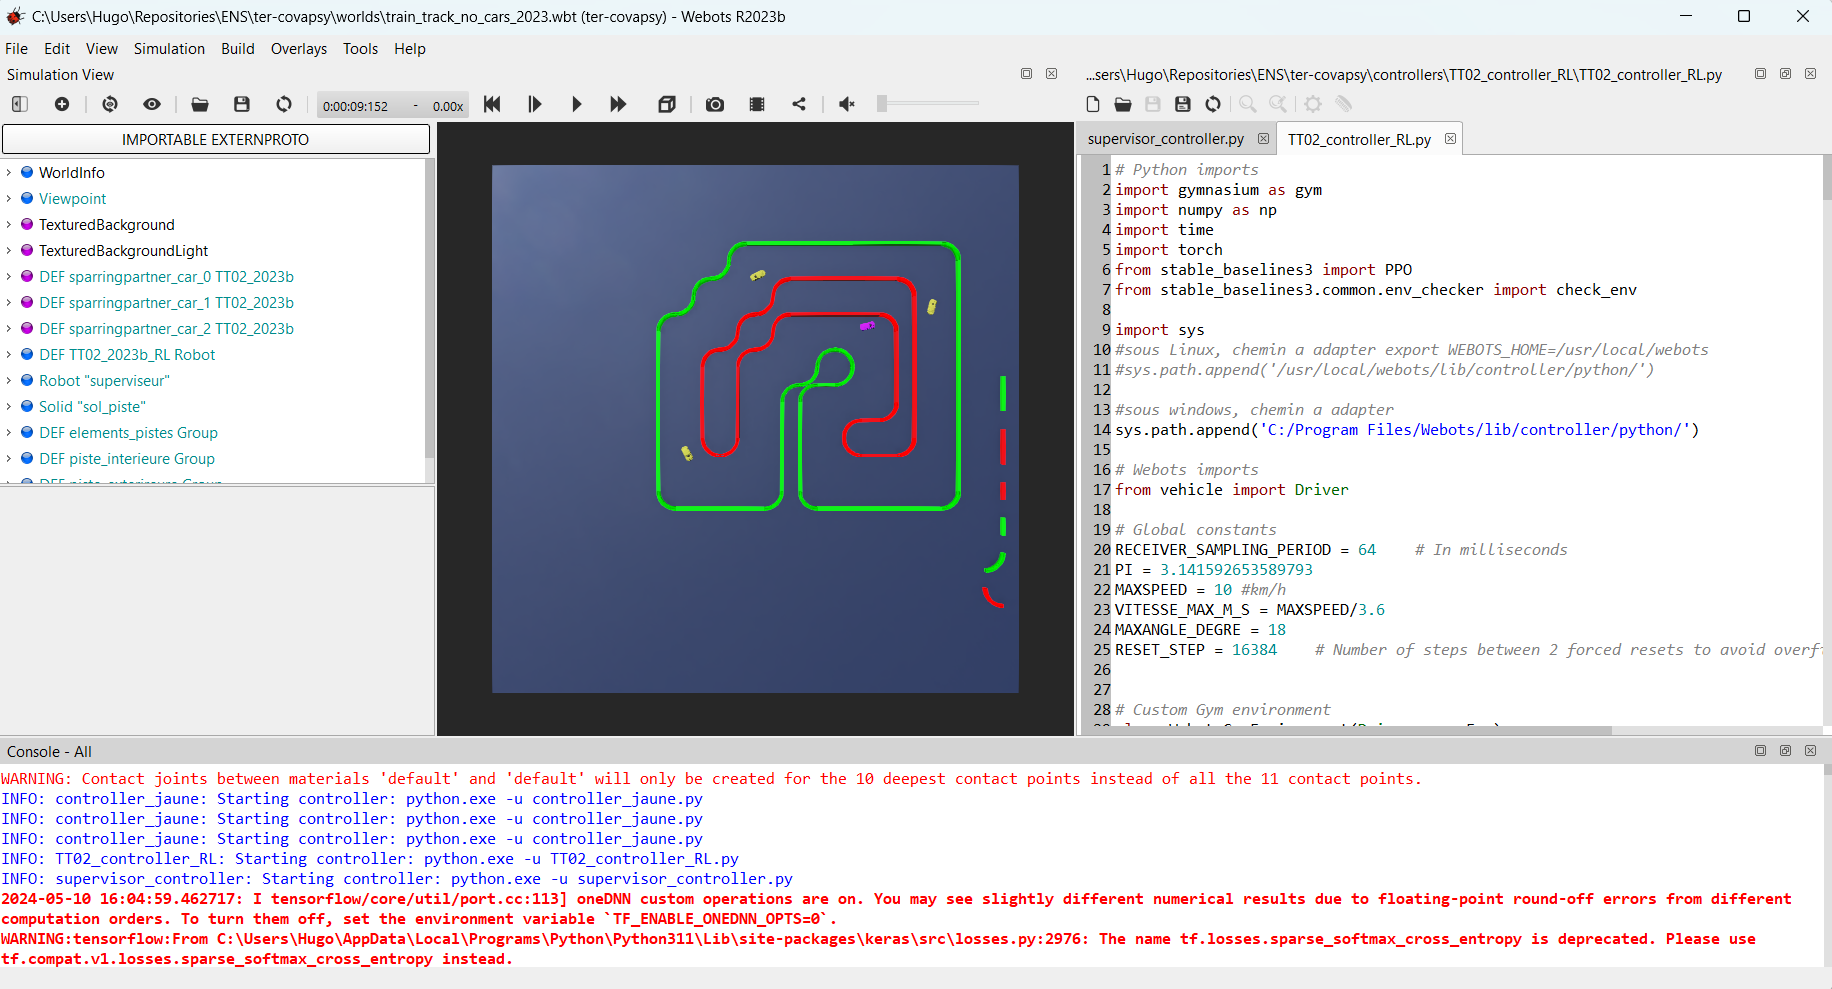
\includegraphics[width=0.9\textwidth]{Images/Webots.png}
    \caption{Capture d'écran de Webots}
\end{figure}


\subsection{Le circuit}
Le circuit dans l'environment de Webots a pour but de simuler un circuit réel sur lequel la voiture autonome doit
apprendre à conduire. Les murs du circuit sont composés de blocs de couleur différentes pour les bordures extérieur et 
intérieur du circuit. Ces murs ont une auteur d'une dizaine de centimètres qui permettent au lidar de mesurer la distance
entre la voiture et les murs.

\begin{figure}[H]
    \centering
    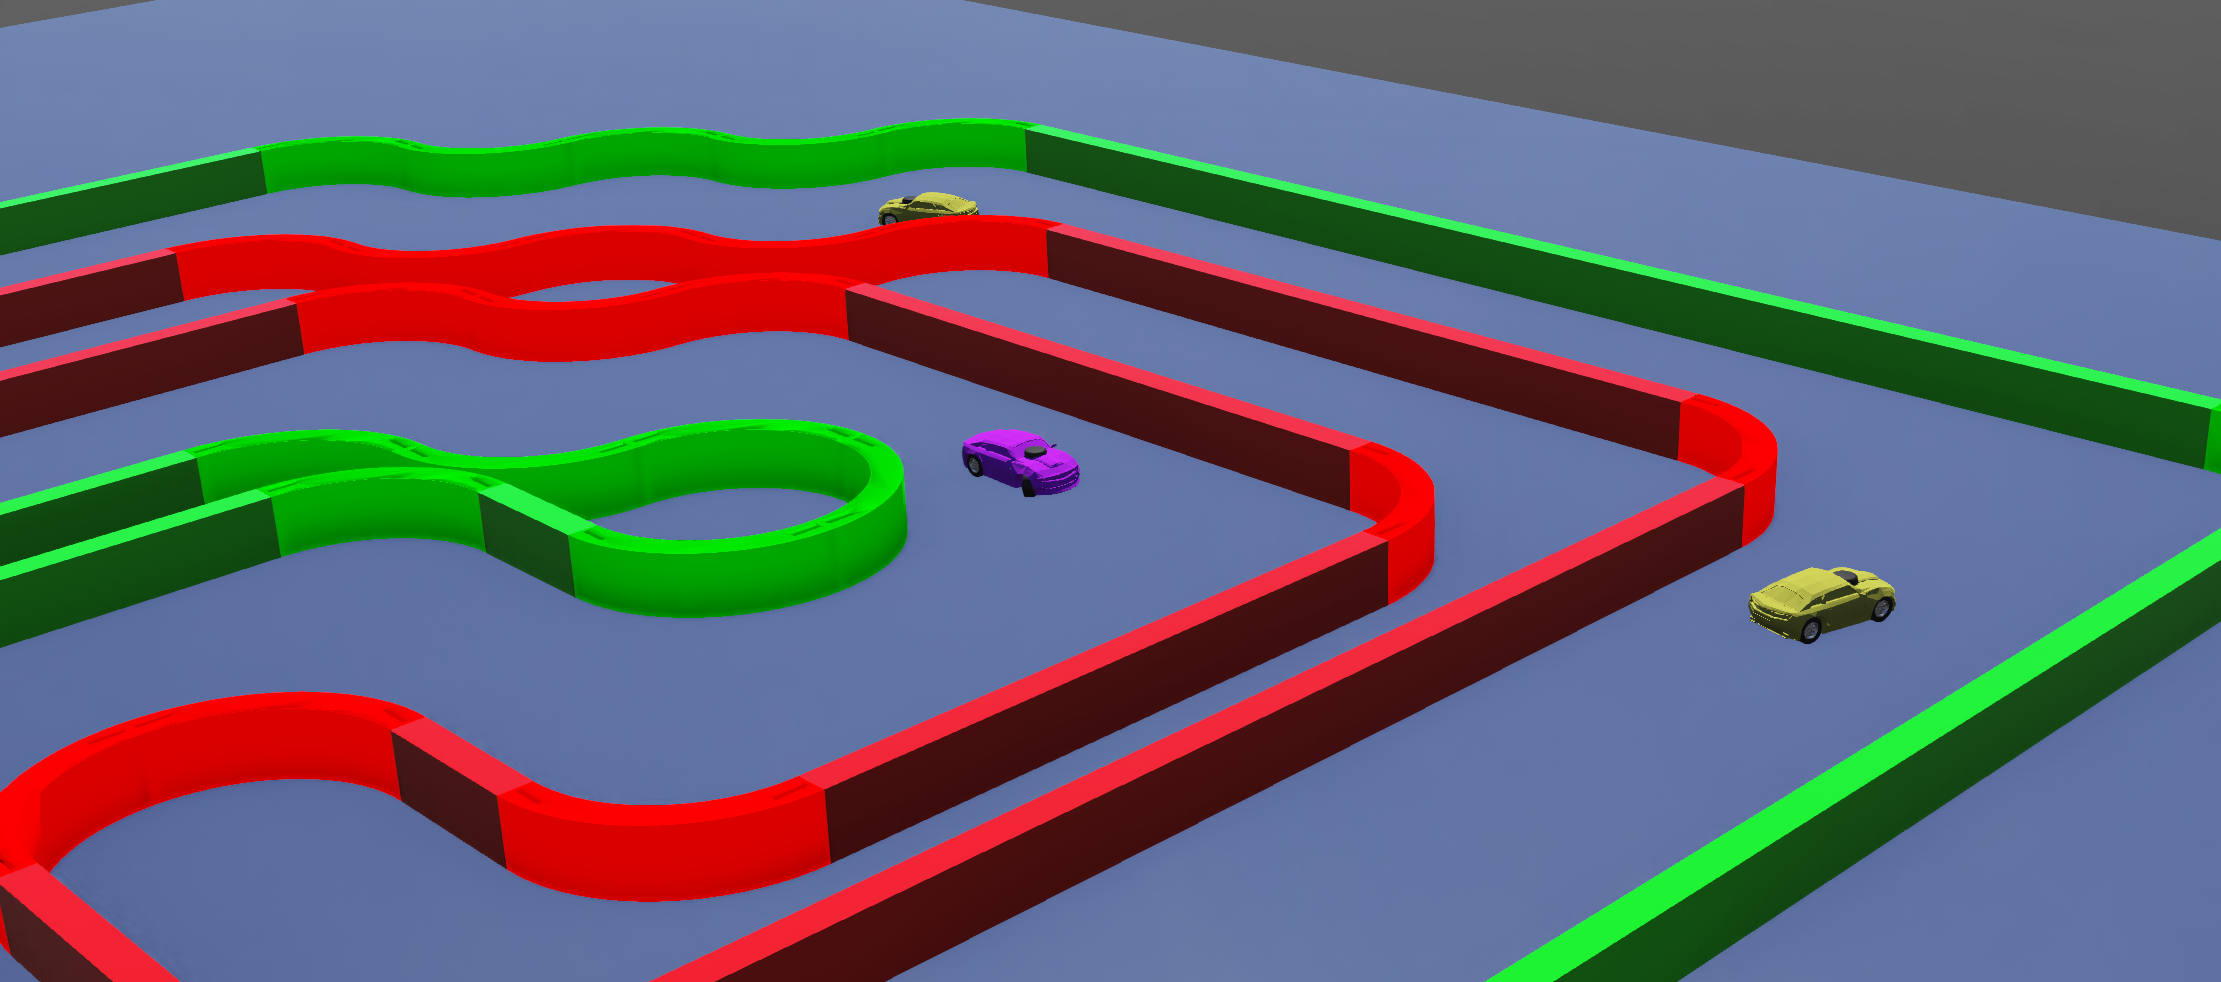
\includegraphics[width=0.9\textwidth]{Images/Circuit.png}
    \caption{Capture d'écran du circuit}
\end{figure}



\subsection{La voiture}
La voiture utilisée dans le simulateur est une voiture RC au format $1/10^{\text{ème}}$. Elle a pour objectif de
reproduire le plus fidèlement possible une voiture réelle. La voiture est équipée d'un lidar qui permet de mesurer la
distance entre la voiture et les murs du circuit à 360 degrés avec une résolution de 1 degré.

\begin{figure}[H]
    \centering
    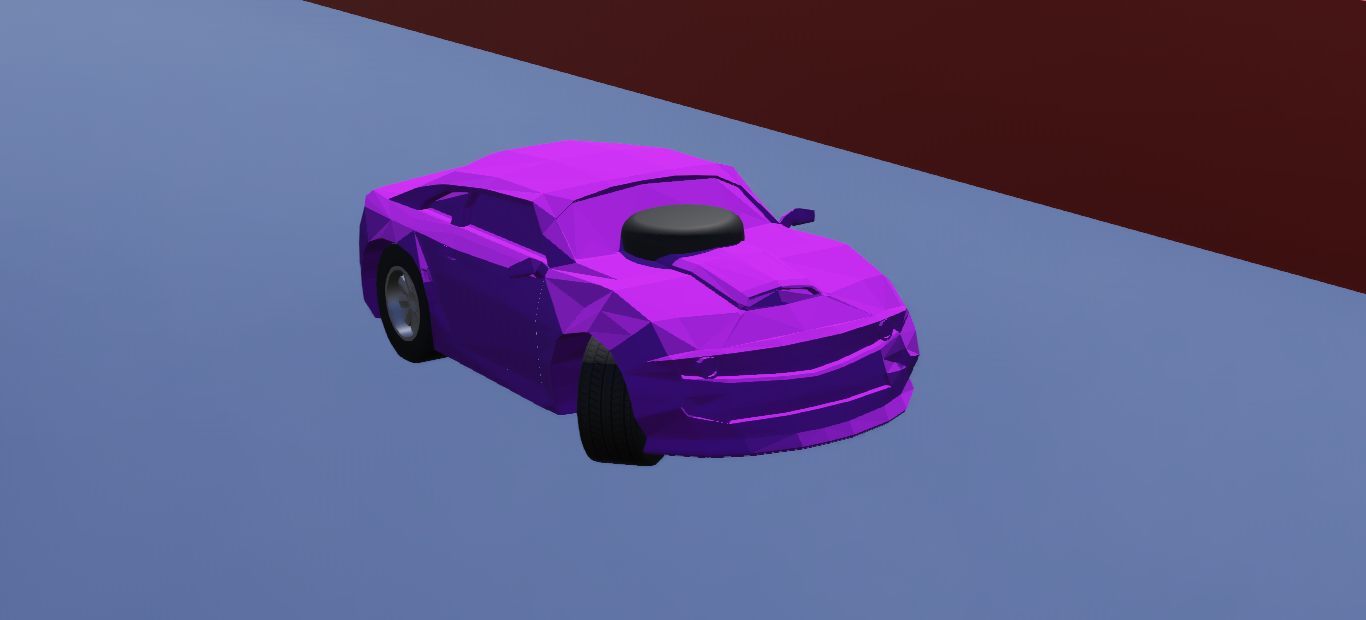
\includegraphics[width=0.9\textwidth]{Images/Voiture.png}
    \caption{Capture d'écran de la voiture}
\end{figure}

\subsection{Les secteurs}

Afin de pouvoir comparer différentes fonctions de récompense et mesurer la performance de la voiture il est possible de mesurer le temps au tour de la voiture (à condition qu'elle finisse un tour complet). Plus de précision sont données dans la section \ref{subsec:reward} Comme la voiture met un certain temps à apprendre à conduire et qu'elle ne termine un tour qu'au bout d'un certain temps, il est intéressant de diviser le circuit en secteurs. Les différentes portions du circuit sont représenté sur la figure \ref{fig:secteurs}.

\begin{figure}[H]
    \centering
    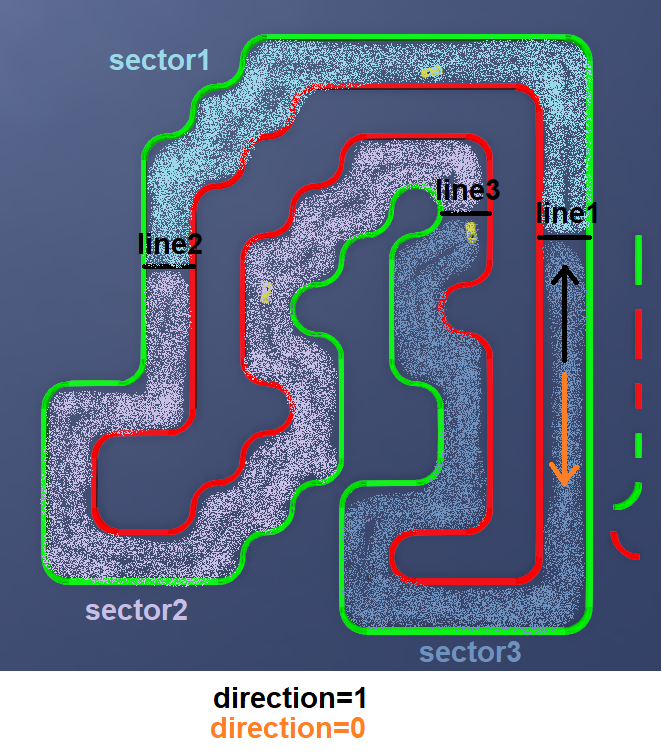
\includegraphics[width=0.9\textwidth]{Images/sector_lines_map.png}
    \caption{Capture d'écran des secteurs}
    \label{fig:secteurs}
\end{figure}

Afin de calculer les temps, on doit pouvoir accéder à la position de la voiture. Or la position n'est accessible qu'au superviseur webots. Pourtant nous avons besoin de cette information dans le controller de la voiture (\verb|TT02_RL_controller.py|) car c'est là qu'est défini la fonction reward et nous souhaitons pouvoir utiliser ces informations de temps au tours/secteurs pour calculer une récompense.
\vspace{0.5cm}

Webots ne permet pas de définir des variables globales ou d'importer des variables définies dans d'autres fichiers dans un soucis de modélisation : dans le monde réel la voiture ne peut pas accéder à sa position si elle n'a pas les capteurs nécessaires. Pour contourner ce problème, nous avons ajouter au controller ansi qu'à la voiture (qui sont tous deux des objets \verb|robots| dans Webots) des émetteurs/receiver. \vspace{0.5cm}

Ainsi on indique à la simulation que notre voiture est munie d'un capteur radio capable de recevoir des informations du controller, notamment ses temps au tours. Ces récepteurs sont nommés \verb|LapEmitter| et \verb|LapReceiver| dans les codes \verb|supervisor_controller.py| et \verb|TT02_RL_controller.py| disponibles \href{https://github.com/basileplus/RCAutonomousCar.git}{ici} dans le dossier \verb|simulatedCar/webotsWorld/controllers|.

\vspace{0.5cm}

La même mécanique est utilisée pour que la réinitialisation lors d'un crash : le superviseur a besoin des données lidar pour savoir si la voiture a crashé. Ces données sont envoyées par la voiture au superviseur via un émetteur/recepteur nommé \verb|resetEmitter| et \verb|resetReceiver|.

\vspace{0.5cm}

Les performances de la voiture (temps au tour,secteur etc.) sont directement affichable dans tensorboard (figure \ref{fig:tensorboard}).

\begin{figure}[H]
    \centering
    \includegraphics[width=0.9\textwidth]{Images/tensorboard.png}
    \caption{Capture d'écran de tensorboard}
    \label{fig:tensorboard}
\end{figure}

Pour ouvrir tensorboard il suffit de :
\begin{itemize}
    \item ouvrir une invite de commande depuis le dossier controller TT02
    \item Executer la commande suivante :
    \begin{minted}{bash}
    python3 -m tensorboard.main --logdir PPO_Tensorboard/
    \end{minted}
    \item Récupérer l'adresse https donnée par la console et la coller dans un navigateur
\end{itemize}


\section{Simulation to real world}

\subsection{Le problème du SimToReal}

L'objectif du SimToReal est de transférer un réseau de neurones entraîné sur un simulateur à une voiture réelle. 
Une fois le réseau de neurones entraîné, il est transféré à la voiture réelle pour qu'elle puisse conduire de manière autonome sur un circuit réel. Un des principaux défis du SimToReal est d'éviter d'avoir une voiture dont les performances sont bonnes sur simulateur mais mauvaises sur la voiture réelle.


\vspace{0.5cm}
L'entraînement sur simulateur a beaucoup d'avantages. Tout d'abord, il permet de réduire le temps et le coût
de l'entraînement. En effet, il est possible de simuler des milliers d'épisodes en quelques heures 
alors qu'il faudrait plusieurs jours pour réaliser le même nombre d'épisodes sur une voiture réelle. De plus,
la simulation permet de tester des scénarios dangereux pour la voiture sans risquer de l'endommager.
Sur la voiture réelle, il faut aussi la replacer à la main après chaque crash dans un mur. Il est donc plus
efficace de réaliser l'entraînement sur simulateur.

\vspace{0.5cm}

Plusieurs solution on été explorées pour améliorer le passage du simulateur à la voiture réelle. Nous allons les détailler dans la suite de cette section. Nous avons implémenté  un certain nombre de fonctions dans le but de randomiser le domaine (\textit{domain randomization}). En ajoutant de l'aléatoire à la simulation on évite d'overfitter le cadre proposé dans le simulateur, et le modèle est capable de répondre à un environnement variable et imparfait. Ainsi le modèle est plus robuste et le passage sim2real est facilité\cite{tobin2017domain}.

\vspace{0.5cm}

Voici les fonctionnalité que nous allons détailler plus bas :
\begin{itemize}
    \item Amélioration de la ressemblance entre le simulateur et le monde réel
    \item Ajout de bruit de mesure
    \item Ajout d'aléatoire dans les commandes
    \item Ajout d'obstacles aléatoires
\end{itemize}

\subsection{Amélioration de la resssemblance entre le simulateur et le monde réel}
\subsection{Amélioration de la ressemblance entre le simulateur et le monde réel}

\subsubsection{Amélioration de la simulation}

La première solution pour améliorer le passage du simulateur à la voiture réelle est d'avoir une simulation et un monde réel les plus proches possibles. Dans cet effort, deux solutions sont possibles :
\begin{itemize}
    \item Améliorer la simulation pour qu'elle soit la plus proche possible de la réalité.
    \item Modifier le monde réel pour qu'il soit le plus proche possible de la simulation.
\end{itemize}

\vspace{0.5cm}
Pour améliorer la simulation, on peut jouer sur différents paramètres du moteur physique. Par exemple, dans la simulation initiale de Webots, le couple des moteurs de direction est de 1e4 Nm ce qui n'est pas réaliste.
Le moteur physique de Webots est puissant et les paramètres par défaut ne sont pas réalistes.
Il est par exemple possible d'ajouter des coefficients de frottements entre les pneus et le sol via \verb|WorldInfo| -> \verb|contactProperties|. Il suffit ensuite de remplir les champs \verb|contactMaterial| des objets \verb|Solid "sol_piste"| et \verb|wheel|.
\vspace*{0.5cm}

Toutefois la modification des paramètres physiques de la simulation est délicate et des comportement inattendus apparaissent très souvent. Par exemple l'observation des roues se désagrégeant après quelques secondes de simulation lorsque des frottements sont simulés.
\vspace*{0.5cm}

On peut toutefois lister quelques paramètres modifiables pour améliorer la simulation:
\begin{itemize}
    \item \textbf{Coefficient de frottement} : Il est possible d'ajouter/modifier le coefficient de frottement entre les roues et le sol pour que la voiture glisse plus ou moins.
    \item \textbf{Masse de la voiture} : La masse de la voiture peut être modifiée.
    \item \textbf{Puissance des moteurs} : Le couple et la vitesse max des moteurs peut être augmentée ou diminuée.
    \item \textbf{Le nombre de roues motrices} : Selon la voiture réelle utilisée, il peut être nécessaire de modifier le nombre de roues motrices.
    \item \textbf{Angle de braquage des roues} : L'angle de braquage des roues peut être modifié pour que la voiture puisse tourner plus ou moins.
    \item \textbf{Lidar} : Les paramètres du Lidar peuvent être modifiés.
\end{itemize} 

\subsubsection{Correction sur la voiture réelle} \vspace{0.5cm}

Il est aussi possible de jouer sur certains paramètres physiques réels. Les \textbf{moteurs} Dynamixel utilisés pour la direction sont configurables via \href{https://emanual.robotis.com/docs/en/software/dynamixel/dynamixel_wizard2/}{Dynamixel Wizard}
\vspace{0.5cm}

Il est très important de faire tourner la voiture réelle une fois la simulation prise en main pour prendre conscience des ces écarts simulation/réalité et essayer de les corriger. Certains sont propres à la voiture et peuvent être corrigés directement via le code python de contrôle de la voiture. 

\vspace{0.5cm}

\paragraph{Lidar}
En testant le bon fonctionnement du \textbf{Lidar}, nous avons constaté que certains points Lidar valaient 0 dans une zone dégagée. Dans ce cas, nous avons implémenté une simple interpolation linéaire pour remplacer ces valeurs par des valeurs cohérentes.

\paragraph{Batterie}
Le niveau de la \textbf{batterie} influence aussi beaucoup la réactivité des moteurs. Si c'est un paramètre qui peut être pris en compte dans la simulation, s'assurer d'utiliser une batterie chargée pour les tests réels est une solution plus efficace.

Nous avons identifié les performances suivantes :

\begin{table}[H]
    \centering
    \begin{tabular}{|c|c|}
        \hline
        \text{Batterie vide} & 0.8 m/s en imposant 1 m/s \\
        \hline
        \text{Batterie pleine} & 2.3 m/s en imposant 1 m/s \\
        \hline
        \text{Vitesse max batterie pleine} & 10 m/s \\
        \hline
    \end{tabular}
\end{table}

\paragraph{Moteur de direction}

Les \textbf{angles de braquage} peuvent être étudiés sur la voiture réelle. La commande du moteur de direction utilisé sur la voiture réelle (\href{https://emanual.robotis.com/docs/en/dxl/ax/ax-12w/}{Dynamixel AX12}) se fait via l'envoie d'un nombre entier. Les commandes dépendent des paramètres de configuration sur Dynamixel Wizard. Il existe deux butées pour les moteurs :
\begin{itemize}
    \item Une butée mécanique qui empêche le moteur de tourner plus loin sur le système de direction.
    \item Une butée logicielle qui empêche le moteur de tourner plus loin que la valeur maximale ou minimale configurée (configurable sur Wizard)
\end{itemize}

Selon le système de direction utilisé les angles de braquage limites ne sont pas les mêmes. Pour \verb|voitureBasile| les angles sont de -18° et 18°. 

Les paramètres identifiés sont :
\begin{table}[H]
    \centering
    \begin{tabular}{|c|c|}
        \hline
        \text{Angle souhaité} & \text{Commande moteur} \\
        \hline
        \text{-18° (butée gauche)} & 300 \\
        \hline
        \text{0° (milieu)} & 460 \\
        \hline
        \text{18° (butée droite)} & 570 \\
        \hline
    \end{tabular}
    \caption{Commande moteur à imposer en fonction de l'angle de direction souhaité}
    \label{tab:commande}
\end{table}

Comme on peut le constater la commande n'est pas linéaire et la plage -18° à 0° est plus grande que la plage 0° à 18°. Nous verrons dans la section \ref{sec:entrainement} comment prendre en compte ces non linéarités dans l'entraînement.

\vspace{0.5cm}

Les paramètres du moteur de direction peuvent être testés via le code \verb|test_direction_AX12.py| disponible \href{https://github.com/basileplus/RCAutonomousCar.git}{ici}
    

\paragraph{Moteur de propulsion}

Le moteur de propulsion utilisé est commandé via un signal PWM. 
Le test du moteur de propulsion se fait via le code \verb|test_propulsion.py| disponible \href{https://github.com/basileplus/RCAutonomousCar.git}{ici}. Les performances identifiées sont les suivantes :

\begin{table}[H]
    \centering
    \begin{tabular}{|c|c|}
        \hline
        Paramètre        & Valeur \\
        \hline
        Point zéro       & 7.09  \\
        \hline
        Point mort       & 0.399 \\
        \hline
        Delta prop max   & 1.5   \\
        \hline
    \end{tabular}
\end{table}

\vspace*{0.5cm}

Pour ces raisons un entraînement sur simulateur est inévitable. 


\subsection{Ajout de bruit}
Un entraînement supplémentaire de la voiture réelle pourrait s'avérer très pertinent en plus de l'entraînement sur simulation pour améliorer le passage sim2real. Dans ce cas, une voie d'exploration est d'utiliser un modèle de type Progressive Neural Network, qui permet au modèle d'intelligemment utiliser ses connaissances acquises sur simulateur tout en continuant d'apprendre sur le circuit réel \cite{rusu2022progressive}. 

\vspace{0.5cm}

Pour les voitures travaillant avec la vision, les images issues de la simulation sont encore plus éloignées des images de la caméra réelle que ce n'est le cas pour le Lidar. Il existe des architectures de modèles combinant CNN et vision transformer construits pour se concentrer sur les parties importantes de l'image et qui possèdent des bonnes capacités de généralisation \cite{li2023style}.

\vspace{0.5cm}

Utiliser une simulation plus simple pourrait améliorer le passage sim2real. Webots est un moteur physique complexe et en plus d'être complexe à manipuler, il est difficile de comprendre les comportements inattendus. Il semblerait qu'une simulation très simpliste comme présentée dans \href{https://www.youtube.com/watch?v=Cy155O5R1Oo&list=PLg2V2juOLiPWxd5fQOz1la37etAf9_WoW&index=4}{cette vidéo} pourrait présenter de meilleures performances, en plus d'être plus accessible. Cette idée selon laquelle le passage sim2real est améliorer lorsque la simulation est plus réaliste (et donc plus complexe) est contredite par les résultats de \cite{pmlr-v205-truong23a} qui montrent que des simulations plus simples peuvent être plus efficaces pour le passage sim2real.

\subsection{Introduction du bruit pour améliorer la simulation}
Pour améliorer le passage sim2real l'ajout de bruit est très efficace. En effet, les modèles de réseaux de neurones sont très sensibles aux données d'entrée. Si les données d'entrée sont trop propres, le modèle risque de surapprendre sur ces données et de ne pas généraliser sur des données plus bruitées.\vspace{0.5cm}

Ces bruits peuvent intervenir à deux niveau :
\begin{itemize}
    \item les mesures des capteurs 
    \item les actions de la Voiture
\end{itemize}

\subsubsection{Bruit sur les mesures}
Dans un environnement réel, les capteurs ne fournissent pas des mesures parfaites. Les mesures du Lidar peuvent 
toujours être affectées par de petites interférences ou des variations mineures. Pour simuler ces conditions, 
on peut ajouter un léger bruit gaussien aux mesures du Lidar. Cela permet au réseau de neurones de s'adapter 
à des données moins parfaites, similaires à celles qu'il rencontrera dans le monde réel. Cette approche n'a pas encore été étudiée, nous avons considéré que les mesures du Lidar étaient suffisamment consitentes.


\subsubsection{Bruit sur les actions}

Les actions de la voiture, telles que l'angle de direction ou la vitesse, sont sujettes à des 
variations imprévues. Par exemple, un servomoteur peut ne pas toujours répondre de manière identique à une même 
commande en raison de l'usure ou des variations de tension. Pour prendre en compte ces imperfections, on peut 
ajouter du bruit aux actions commandées par le réseau de neurones. Cela aide à rendre l'agent plus robuste face 
aux variations qu'il pourrait rencontrer sur une voiture réelle. Ainsi lorsque le réseau de neurones est transposé sur la voiture réelle, il ne sera pas surpris si les moteurs ne répondent pas exactement comme dans la simulation.

\vspace{0.5cm}

Les l'espace de commande que l'on obtient en sortie du réseau de neuronnes est un angle de direction et une vitesse. Il y a donc deux champs auxquels on peut ajouter du bruit à chaque itération :
\begin{itemize}
    \item La commande de vitesse
    \item La commande d'angle
\end{itemize}

Ce bruit peut être ajouté dans les fonctions \verb|set_vitesse_m_s| et \verb|set_direction_degre| du fichier \verb|TT02_controller_RL.py|. 

Ainsi à chaque commande en sortie du réseau de neuronne, la voiture ne répondra pas exactement comme attendu mais répondra à une consigne bruitée. \vspace{0.5cm}

Ce type de bruit n'a pas été implémenté. Pour notre étude nous avons préféré nous concentrer sur l'ajout d'aléatoire sur les commandes de la voiture mais non pas à chaque timesteps (cad à chaque nouvelle commande est associé un bruit aléatoire) mais à chaque réinitialisation de la voiture. Cette approche est explicitée dans la sous-section \ref{subsec:random}

\subsection{Ajout d'aléatoire dans les commandes}

\label{subsec:random}

Nous avons implémenté un système de randomisation des directions et des vitesses pour améliorer la robustesse du modèle. A chaque réinitialisation de la voiture, un biais aléatoire est ajouté à la commande de direction et de vitesse. 

L'alétoire peut être activé ou désactivé via la variable \verb|self.add_randomness| dans le fichier \verb|TT02_controller_RL.py|.

\subsubsubsection{Randomisation des directions}

Commençons par décrire comment nous avons modélisé la réponse de la voiture à une consigne d'angle.

\vspace{0.5cm}

\paragraph{Modélisation}

Comme nous l'avons vu dans le tableau \ref{tab:commande} l'angle des roues sur la voiture réelle n'est pas linéairement relié à la consigne moteur (et donc à l'angle du moteur de direction). Ainsi la modélisation suivante a été choisie pour modéliser sur le simulateur quel angle prennent les roues de la voiture en fonction de la consigne d'angle :
\begin{equation}
    \alpha = \left(\frac{b}{324}\right) \theta^2 + \theta + b
\end{equation}
Cette fonction a été tracée figure \ref{fig:angle_com}

\begin{figure}[H]
    \centering
    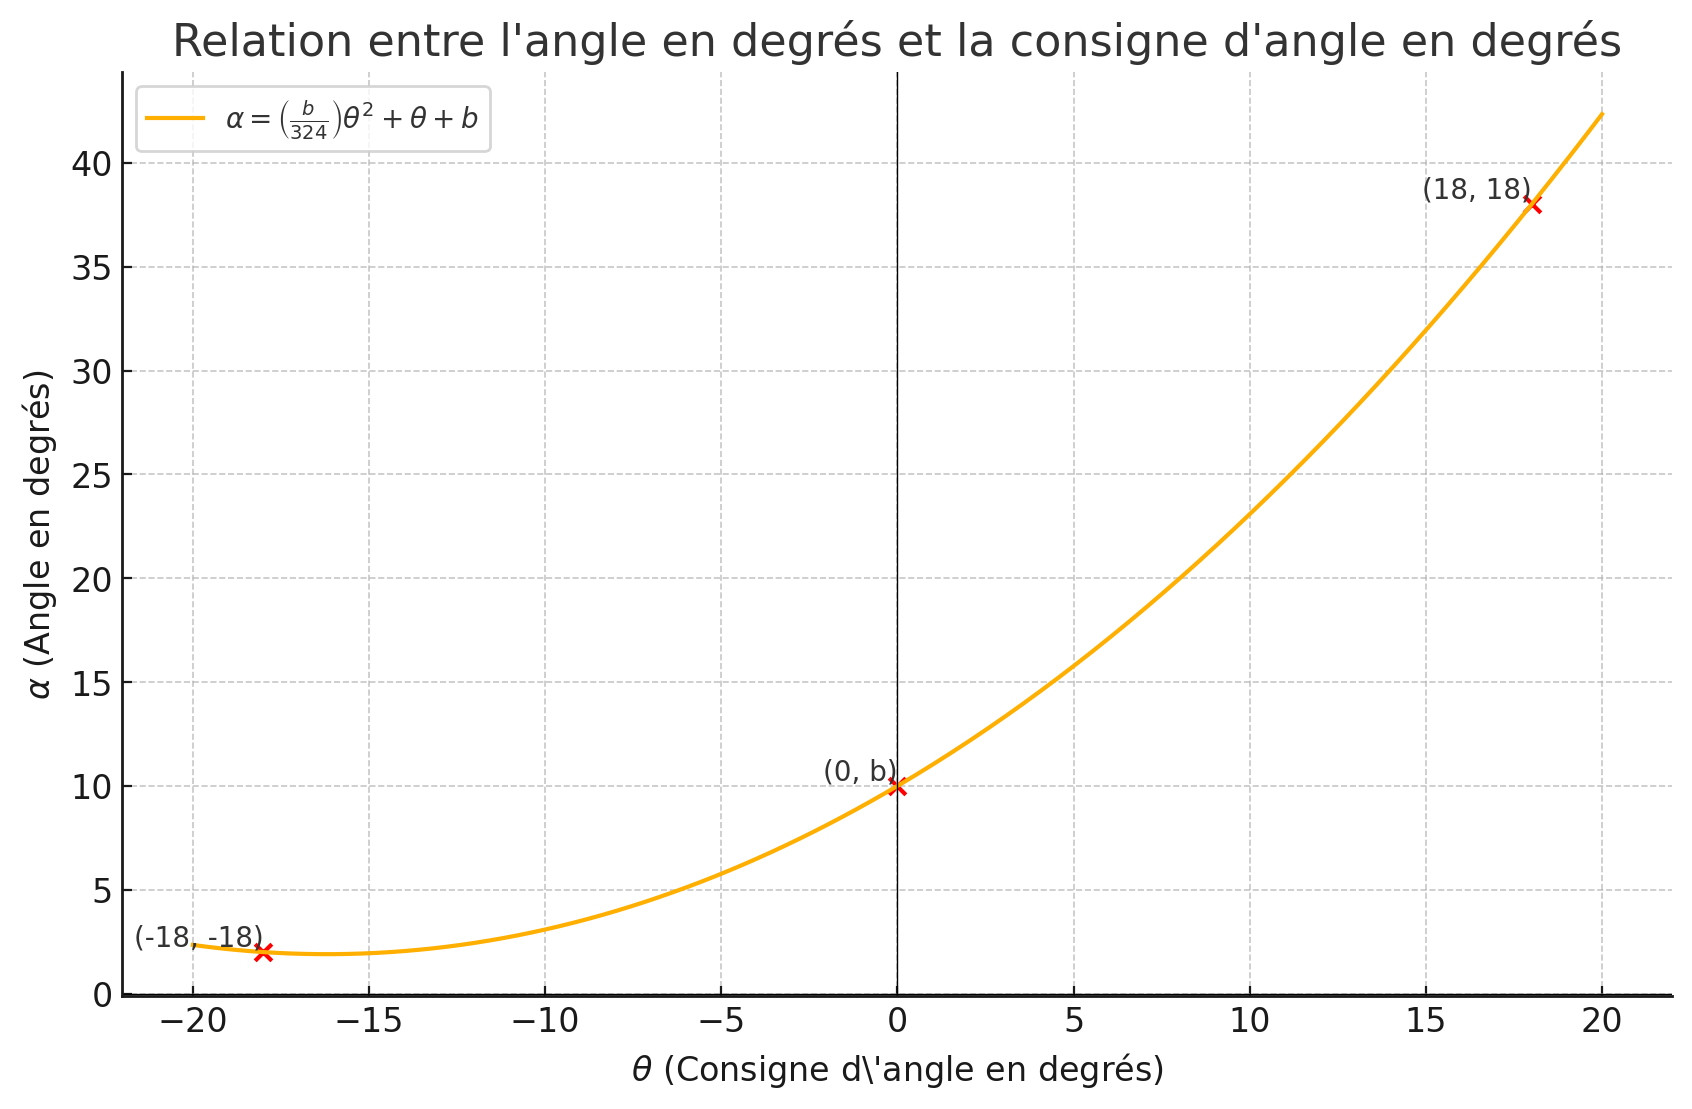
\includegraphics[width=0.6\textwidth]{Images/angle_com.png}
    \caption{Modélisation de l'angle des roues en fonction de la consigne d'angle}
    \label{fig:angle_com}
\end{figure}

\bigskip

où :
\begin{itemize}
    \item \(\alpha\) : L'angle en degrés réellement imposé à la voiture.
    \item \(\theta\) : La consigne d'angle en degrés.
    \item \(b\) : Le biais directionnel, une constante ajoutée pour ajuster l'angle lorsque la consigne est $\theta = 0$.
\end{itemize}

Cette fonction passe par les points $(-18, -18)$, $(0, b)$ et $(18, 18)$.

Ainsi nous respectons les angles de butée de la voiture réelle

\paragraph{Ajout d'aléatoire}

Pour améliorer la robustesse du modèle, à chaque replacement de la voiture, on initialise aléatoirement le paramètre \verb|self.random_dir_bias| qui représente $b$.

La valeur est choisie aléatoirement entre [-\verb|self.max_random_dir_bias|,\verb|self.max_random_dir_bias|]

\subsection{Randomisation des vitesses}

\paragraph{Modélisation}

Pour la vitesse, nous avons choisi de modéliser la réponse de la voiture à une consigne de vitesse de la manière suivante :

\begin{equation}
    v_{\mathrm{out}} = k \cdot v_{\mathrm{in}} + b
\end{equation}

\begin{itemize}
    \item \(v_{\mathrm{out}}\) : La vitesse réellement demandé à la voiture par le simulateur.
    \item \(v_{\mathrm{in}}\) : La consigne de vitesse.
    \item \(k\) : Facteur de proportionnalité.
    \item \(b\) : Le biais ajouté à la vitesse.
\end{itemize}

\paragraph{Ajout d'aléatoire}

Ici aussi, à chaque replacement de la voiture, on initialise aléatoirement le paramètre \verb|self.random_speed_bias| qui représente $b$ ainsi que le paramètre \verb|self.random_speed_prop| qui représente $k$.

\subsection{Ajout d'obstacles aléatoires}

Pour améliorer la robustesse du modèle, nous avons ajouté des obstacles aléatoires sur le circuit (voir figure \ref{fig:random_obs}). Ces obstacles sont des blocs cubiques. Ils sont placés aléatoirement sur le circuit à chaque réinitialisation de la voiture. Leurs positions sont choisies aléatoirement parmis une liste de positions prédéfinies. 

\begin{figure}[H]
    \centering
    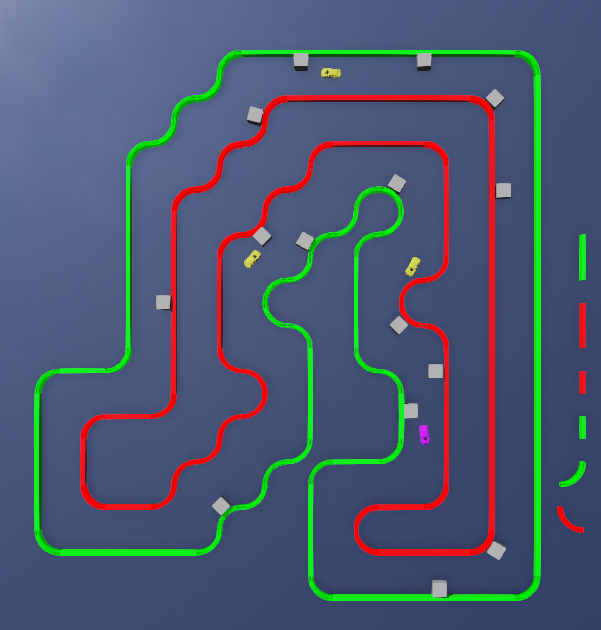
\includegraphics[width=0.6\textwidth]{Images/random_obs.png}
    \caption{Circuit avec obstacles aléatoires}
    \label{fig:random_obs}
\end{figure}

\vspace{0.5cm}
La génération d'obstacles est gérée dans le code \verb|supervisor_controller.py| disponible \href{https://github.com/basileplus/RCAutonomousCar/tree/main/simulatedCar}{ici} dans le fichier \verb|controllers\TT02_controller_RL|. Le nombre d'obstacle à placer peut être modifié directement dans boucle \verb|while| principale à la ligne
\begin{lstlisting}
indexes = random.sample(range(0,len(obstacles_positions)), nb_obstacles)
\end{lstlisting}

L'ajout d'obstacles peut être désactivée via la variable \verb|self.add_obstacle| dans le fichier \verb|supervisore_controller.py|.

\subsection{Position de départ aléatoires}

Tout comme pour les obstacles aléatoires, la voiture démarre à une position aléatoire sur le circuit à chaque réinitialisation. La position de départ est choisie aléatoirement parmis une liste de positions prédéfinies. On ajoute de plus un angle de départ aléatoire pour que la voiture ne démarre pas toujours dans la même direction.


\subsection{Résultats}

Des entrainements avec l'ajout d'aléatoire ont été lancés. Lorsque les paramètres \verb|max_random_dir_bias|, \verb|max_random_speed_prop|, \verb|max_random_speed_bias| et le nombre d'obstacles ne sont pas trop élevés, la voiture est capable de conduire correctement et de faire des tours de circuit.

\vspace{0.5cm}

Le modèle obtenu est donc en théorie beaucoup plus robuste que précédemment pour des performances similaires. Cependant après des tests sur la voiture réelle, il s'avère que le modèle ne performe pas mieux que celui obtenu avant l'ajout d'aléatoire. 
\vspace{0.5cm}

Nous expliquons ce résultat par par un manque d'optimisation du code de la voiture réelle. L'élément limitant les performances de la voiture réelle n'est pas le modèle entrainé sur simulateur mais la façon dont ce modèle est utilisé sur la voiture réelle\footnote{les voitures utilisant le RL les plus performantes lors de la courses sont celles qui ont beaucoup travaillé sur le code voiture} via le code \verb|programme_course.py| disponible \href{https://github.com/basileplus/RCAutonomousCar.git}{ici}. Il semble donc que travailler sur le code de la voiture réelle soit plus pertinent que de continuer d'essayer d'améliorer le modèle.

\subsection{Améliorations possibles}

nous conseillons en premier lieu de travailler sur le code de la voiture réelle pour améliorer les performances de la voiture. En effet, les performances de la voiture réelle sont très loin de celles obtenues sur simulateur. Ci dessous quelques autres pistes d'améliorations que nous n'avons pas pu explorer/implémenter.

\vspace{1cm}

Un entrainement supplémentaire de la voiture réelle pourrait s'avérer très pertinent en plus de l'entrainement sur simulation pour améliorer le passage sim2real. Dans ce cas, une voie d'exploration est d'utiliser un modèle de type Progressive Neural Network, qui permet au modèle d'intelligemment utiliser ses connaissances acquises sur simulateur tout en continuant d'apprendre sur le circuit réel \cite{rusu2022progressive}. 

\vspace{0.5cm}

Pour les voitures travaillant avec la vision, les images issues de la simulation sont encore plus éloignées des images de la caméra réelle que ce n'est le cas pour le Lidar. Il existe des architectures de modèles combinant CNN et vision transformer construits pour se concentrer sur les parties importantes de l'image et qui possèdent des bonnes capacités de généralisation \cite{li2023style}.

\vspace{0.5cm}

Utiliser une simulation plus simple pourrait améliorer le passage sim2real. Webots est un moteu r phyique complexe et en plus d'être complexe à manipuler, il est difficile de comprendre les comportements inattendus. Il semblerait qu'une simulation très simpliste comme présentée dans \href{https://www.youtube.com/watch?v=Cy155O5R1Oo&list=PLg2V2juOLiPWxd5fQOz1la37etAf9_WoW&index=4}{cette vidéo} pourrait présenter de meilleures performances, en plus d'être plus accessible. Cette idée selon laquelle le passage sim2real est améliorer lorsque la simulation est plus réaliste (et donc plus complexe) est contredite par les résultats de \cite{pmlr-v205-truong23a} qui montrent que des simulations plus simples peuvent être plus efficaces pour le passage sim2real.



\section{Application à la voiture autonome}
Pour appliquer l'apprentissage par renforcement à une voiture autonome, nous devons définir correctement 
l'espace d'observation et l'espace d'action en tenant compte des contraintes du monde réel. En effet, 
tout ce qui est possible dans un simulateur n'est pas forcément réalisable dans le monde réel. 

\subsection{Espace d'action}
L'espace d'action est limité aux commandes que l'agent peut envoyer à la voiture. Cela inclut:
\begin{itemize}
    \item La vitesse de la voiture
    \item L'angle de direction de la voiture
\end{itemize}
Dans notre cas, les actions seront le fait d'augmenter ou de diminuer les consignes de vitesse et d'angle de direction.


\subsection{Espace d'observation}
L'espace d'observation doit inclure toutes les informations pertinentes que la voiture peut obtenir de son environnement.
Dans notre cas, le Lidar pour mesurer les distances aux obstacles. Si un système de contrôle de 
la vitesse est en place, la vitesse actuelle de la voiture pourrait également faire partie de l'espace d'observation. 

\vspace{0.5cm}
Dans notre cas nous avons donné les données du lidar à l'instant présent et à l'instant précédent, cela permet
de donner une information sur la vitesse de la voiture et une certaine inertie à la voiture. Nous avons également
les ancienne consignes de vitesse et d'angle de direction pour donner une information sur la dynamique de la voiture.


\section{Entraînement du réseau de neurones}
\subsection{Algorithme d'apprentissage}
\subsubsection*{Circuit d'entraînement}
La piste d'entraînement utilisée est conçue pour offrir une variété de situations afin que la voiture puisse 
apprendre à gérer différentes circonstances qu'elle pourrait rencontrer en course. Le circuit est composé de virages 
à gauche et à droite, de longues lignes droites, de virages en épingle et d'une section en diagonale. 
La piste retenue est la suivante:

\begin{figure}[H]
\centering
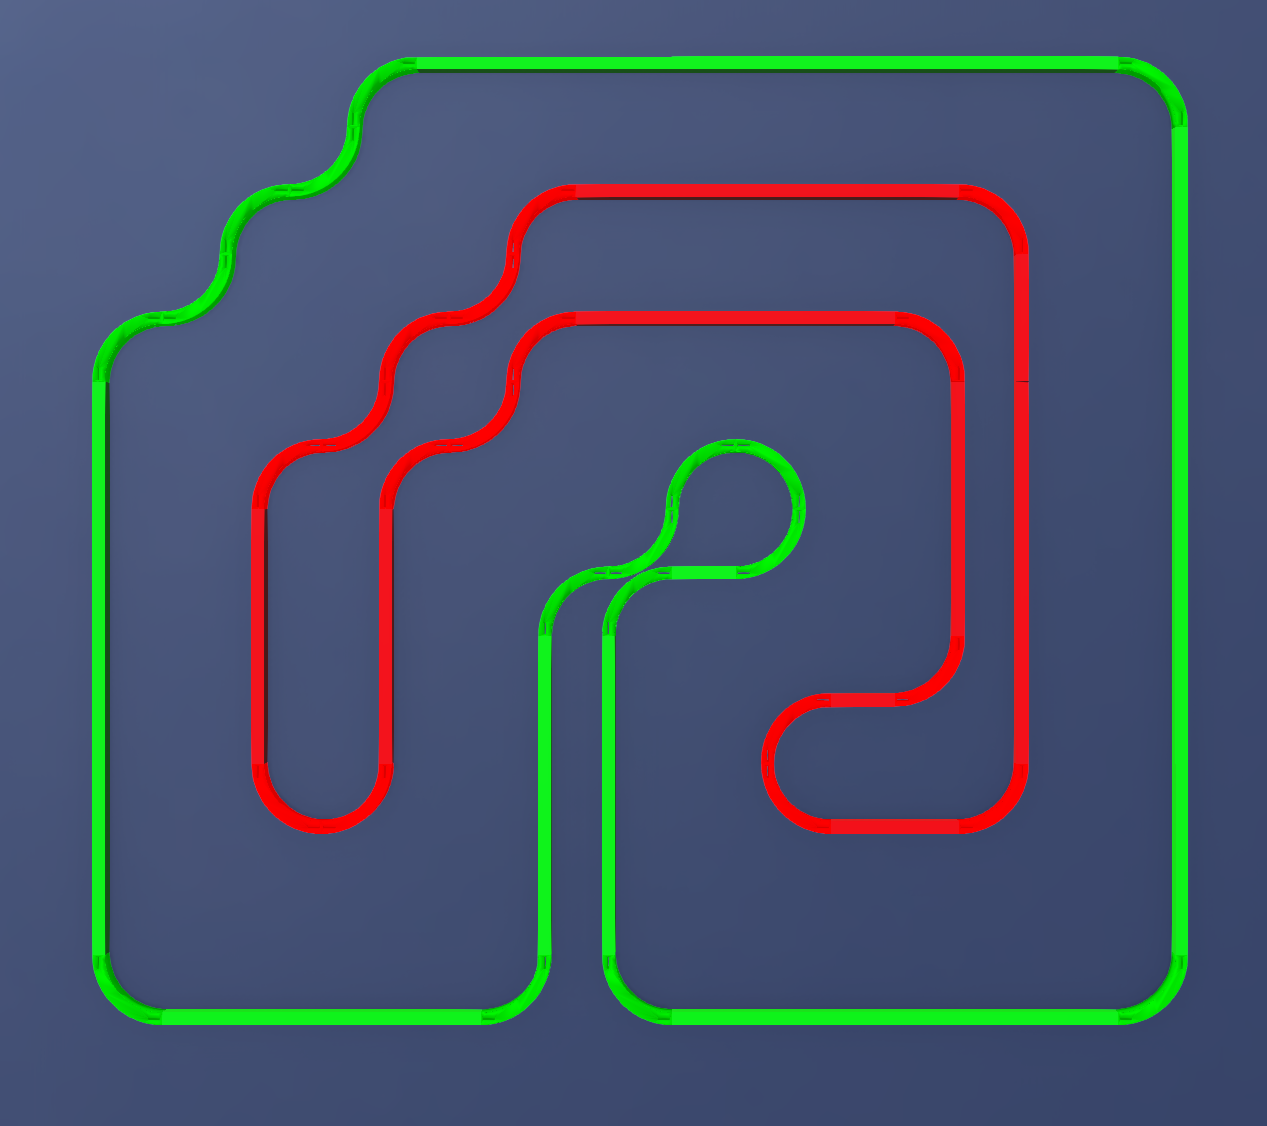
\includegraphics[width=0.8\textwidth]{Images/Piste Entrainement.png}
\caption{Piste d'entraînement pour l'apprentissage par renforcement}
\end{figure}

Sur ce circuit, nous avons ajouté trois autres voitures qui roulent à vitesse modérée pour simuler des situations 
de dépassement. Ces voitures suivent un algorithme de conduite simple qui consiste à rester à distance des murs.

\vspace{0.5cm}
Pour cet environnement, nous avons également intégré un robot "Superviseur" qui repositionne les voitures à des 
positions aléatoires lorsque nous souhaitons recommencer un épisode. Ce "Superviseur" choisit aléatoirement 
une position et une direction sur le circuit pour replacer les voitures, assurant ainsi une situation initiale 
nouvelle à chaque début d'épisode. La communication avec le "Superviseur" se fait via un système émetteur-récepteur 
intégré dans Webots.


\subsubsection*{Environment Gym}
La bibliothèque Gym est une bibliothèque implémentée en Python qui permet de gérer la partie apprentissage par 
renforcement d'un réseau de neurones. Dans le cas de notre projet, Gym ne propose pas d'environnement adapté. 
Il a donc été nécessaire de créer un tout nouvel environnement. Gym exige qu'un environnement contienne les fonctions 
suivantes:
\begin{itemize}
    \item \textbf{get\_observation()} : fonction renvoyant les observations de l'environnement
    \item \textbf{get\_reward()} : fonction donnant la récompense selon l'action effectuée par l'agent
    \item \textbf{reset()} : fonction donnant la démarche pour repartir au début d'un épisode
    \item \textbf{step()} : fonction faisant évoluer l'environnement
\end{itemize}

\vspace{0.5cm}
Toutes ces fonctions sont rassemblées dans une classe que nous avons nommée \texttt{WebotsGymEnvironment}. Dans cette classe, nous avons rajouté quatre fonctions propres à la voiture :
\begin{itemize}
\item \textbf{get\_lidar\_mm()} : Fonction qui renvoie un tableau de Lidar dans le bon format avec des valeurs cohérentes en mm.
\item \textbf{set\_vitesse\_m\_s()} : Fonction qui prend en argument une vitesse en m/s et qui la convertit en km/h avant de l'envoyer à la voiture.
\item \textbf{set\_direction\_degre()} : Fonction qui prend un angle en degré et le convertit en radian avant de l'envoyer à la voiture.
\end{itemize}
\noindent
Nous allons détailler par la suite chacune des fonctions.

\subsubsection*{get\_observation()}
Dans la fonction \texttt{get\_observation()}, on appelle la fonction \texttt{get\_lidar\_mm()} pour récupérer 
les observations du Lidar. Ce tableau sera le tableau donné en entrée du réseau pour les observations du Lidar 
à "l'instant présent". Pour ce qui est du tableau à "l'instant précédent", on stocke à chaque appel de la 
fonction le tableau d'observation dans une variable interne de la classe. Si la fonction est appelée depuis 
la fonction \texttt{reset()}, on donne le même tableau pour les deux parties de l'espace d'observation concernant 
le Lidar puisque la voiture a été repositionnée. Pour la vitesse et la direction, Webots nous permet de mesurer 
la vitesse et la direction de la voiture dans le simulateur. Ce sont ces données que l'on donne au réseau de neurones. 
De même dans le cas où l'observation est demandée par la fonction \texttt{reset()}, on indique que ces deux grandeurs 
sont nulles. Il est à noter que les valeurs données à l'espace d'observation sont normalisées.

\subsubsection*{get\_reward()}

\label{subsec:reward}
Dans la fonction \texttt{get\_reward()}, on donne la récompense associée à l'état dans lequel se trouve la voiture. 
On distingue deux états possibles pour la voiture. Le premier état est celui d'une situation de collision. 
On regarde la plus petite valeur du tableau de Lidar actuel et si celui-ci est inférieur à 120 mm, on considère 
qu'il y a collision. Dans le cas de la collision, on donne un malus de -400 moins la vitesse de la voiture. 
Le deuxième état regroupe toutes les situations autres que celle de collision. On donne comme récompense ici 
une valeur dépendant de la vitesse actuelle de la voiture ainsi que la distance minimale donnée par le tableau de Lidar. 
Les fonctions de récompenses seront détaillées plus tard. On indique aussi ici si l'on a terminé l'épisode via la 
variable \texttt{done}.

Afin de pouvoir une metrics cohérente entre différentes fonctions de récompenses, il est possible de mesurer le temps au tour et au secteur de la voiture. Ainsi on peut comparer différentes fonctions de récompenses et mesurer la performance de la voiture. Plusieurs autre paramètres ont été ajoutés, comme le nombre de collisions, le nombre de tours, le nombre de secteurs, le temps total, le meilleur temps au tour. Tout est affichable 

\subsubsection*{reset()}
Dans la fonction \texttt{reset()}, on indique la démarche à suivre lorsque l'on veut retourner au début d'un épisode. 
Le reset se fait dans le cas d'un crash de la voiture ou si le nombre d'actions autorisées par épisode est atteint. 
Au moment du reset, on donne des consignes de vitesse et d'angle nuls et on envoie une indication de reset au robot 
"Superviseur". À la fin de la routine de réinitialisation, on renvoie une observation.

\subsubsection*{step()}
Dans la fonction \texttt{step()}, on indique que l'on fait un pas dans le processus d'apprentissage. Dans cette 
fonction, on fait avancer la voiture avec les actions récupérées depuis le réseau de neurones. Ensuite, on récupère 
une observation depuis le Lidar et on fait faire un pas au processus d'apprentissage. On calcule la récompense 
avant de retourner toutes les informations obtenues.

\subsection{Réseau de neurones avec Stable-Baselines3}
La librairie Stable-Baselines3 permet de créer un réseau de neurones géré par l'algorithmes d'apprentissage 
par renforcement PPO (Proximal Policy Optimization). Stable-Baselines3 propose un large choix de paramètres pour 
l'apprentissage. Voici un descriptif des paramètres utilisés ainsi que leurs valeurs définies dans notre programme:
\begin{itemize}
    \item \textbf{policy} : Type de politique utilisée. Dans notre cas, nous utilisons 'MultiInputPolicy' 
    pour gérer les multiples entrées.
    \item \textbf{env} : Environnement d'apprentissage Gym.
    \item \textbf{learning\_rate} : Taux d'apprentissage fixé à $5 \cdot 10^{-4}$.
    \item \textbf{n\_steps} : Nombre d'actions autorisées par épisode (2048).
    \item \textbf{batch\_size} : Taille du lot de données pour chaque mise à jour (64).
    \item \textbf{n\_epochs} : Nombre d'époques d'entraînement par itération de \texttt{n\_steps} (10). 
    \item \textbf{gamma} : Facteur de discount pour la récompense future (0.99).
    \item \textbf{gae\_lambda} : Facteur pour le calcul de l'estimateur de l'avantage généralisé (0.95).
    \item \textbf{clip\_range} : Valeur de clipping pour PPO (0.2).
    \item \textbf{vf\_coef} : Coefficient de la fonction de perte de la valeur (1).
    \item \textbf{ent\_coef} : Coefficient d'entropie pour la fonction de perte (0.01).
    \item \textbf{device} : Composant sur lequel faire tourner l'algorithme (dans notre cas, 'cuda:0' pour l'utilisation du GPU).
    \item \textbf{tensorboard\_log} : Emplacement pour enregistrer les données de Tensorboard ('./PPO\_Tensorboard').
\end{itemize}
Voici un extrait de notre code de définition de modèle :
\begin{minted}[
    frame=lines,
    framesep=2mm,
    baselinestretch=1.2,
    bgcolor=LightGray,
    fontsize=\footnotesize,
    linenos
]
{python}
# Définition du modèle
model = PPO(
    policy="MultiInputPolicy",
    env=env,
    learning_rate=5e-4,
    verbose=1,
    device='cuda:0',
    tensorboard_log='./PPO_Tensorboard',
    # Paramètres additionnels
    n_steps=2048,
    batch_size=64,
    n_epochs=10,
    gamma=0.99,
    gae_lambda=0.95,
    clip_range=0.2,
    vf_coef=1,
    ent_coef=0.01
)
\end{minted}

Nous pouvons ensuite entraîner le modèle avec la fonction \texttt{model.learn()}. Cette fonction prend en argument
le nombre d'itérations d'entraînement. Une fois l'entraînement terminé, nous pouvons sauvegarder le modèle avec
la fonction \texttt{model.save()}.Nous pouvons dans un second temps charger le modèle avec la fonction 
\texttt{model.load()} ce qui nous permet, par exemple de reentrainer le modèle avec de nouveau paramètres ou avec 
une nouvelle fonction de récompense. Nous pouvons également visualiser les données d'entraînement avec Tensorboard
en exécutant la commande \texttt{tensorboard --logdir ./PPO\_Tensorboard}.


\subsection{Fonction de récompense}
La fonction de récompense est un élément crucial de l'apprentissage par renforcement. Elle permet de guider
l'agent vers les actions qui maximisent la récompense. C'est un élément délicat à définir car une mauvaise
fonction de récompense peut entraîner des comportements indésirables de l'agent. En effet si l'on ne prend pas 
assez en compte le crash de la voiture, l'agent pourrait apprendre à foncer dans les murs pour maximiser la vitesse.
Si l'on ne prend pas en compte la vitesse, l'agent pourrait apprendre à rester immobile pour éviter les collisions et
rester éloigné des murs. Il est donc important de trouver un équilibre entre ces aspects. 

\vspace{0.5cm}
Dans notre cas, nous avons défini une fonction de récompense qui prend en compte la vitesse de la voiture et la distance
minimale donnée par le Lidar. La récompense est définie comme suit:

\begin{equation}
    \text{reward} = \begin{cases}
        -400 - 10 * \text{vitesse} & \text{si collision} \\
        18 * (\text{mini} - 0.018) + 2 * \text{vitesse} & \text{sinon}
    \end{cases}
\end{equation}

Où $\text{mini}$ est la distance minimale donnée par le Lidar et $\text{vitesse}$ est la vitesse de la voiture.
La récompense est négative en cas de collision et dépend de la vitesse de la voiture. Cela permet de fortement pénaliser
les collisions à haute vitesse. Dans le cas où il n'y a pas de collision, la récompense dépend de la distance minimale
donnée par le Lidar et de la vitesse de la voiture. Cela permet de favoriser les actions qui permettent à la voiture
de rouler vite tout en restant loin des murs pour éviter les collisions.

\vspace{0.5cm}
Nous avons également essayé de prendre en compte le temps de passage au tour. Pour cela, nous avons adapté le 
superviseur afin de détecter les passages sur la ligne d'arrivée et de notifier la fonction de récompense pour 
donner une récompense positive lors d'un passage sur la ligne d'arrivée. Plus le temps au tour est court, plus 
la récompense est élevée. Cela permet de former la voiture à vraiment aller vite et à réaliser un temps au tour 
le plus rapide possible. Cette approche encourage l'agent à optimiser non seulement la vitesse et la sécurité, 
mais aussi l'efficacité globale de ses déplacements sur le circuit.


\subsection{Mise en place de la simulation}
Après avoir défini l'environnement Gym, le réseau de neurones et la fonction de récompense, nous pouvons lancer
l'entraînement de la voiture autonome.

\subsubsection*{Entraînement}
La première étape consiste à déclarer l'environnement Gym et à vérifier que celui-ci est correctement défini avec 
la fonction \texttt{check\_env()}:

\begin{minted}[
    frame=lines,
    framesep=2mm,
    baselinestretch=1.2,
    bgcolor=LightGray,
    fontsize=\footnotesize,
    linenos
]{python}
env = WebotsGymEnvironment()
check_env(env)
\end{minted}

Après cela, nous pouvons définir le modèle et lancer l'entraînement avec la fonction \texttt{model.learn()}. Nous 
donnons en argument \texttt{total\_timesteps} qui correspond au nombre total d'itérations d'entraînement. Nous 
pouvons ensuite sauvegarder le modèle avec la fonction \texttt{model.save()} qui prend en argument le nom du fichier
de sauvegarde.

\section*{Passage à la voiture réelle}
Une fois le réseau de neurones entraîné sur le simulateur, nous pouvons le transférer à la voiture réelle. C'est 
la dernière étape du projet. Cette transition du monde virtuel au monde réel nécessite une adaptation des algorithmes 
et des fonctionnalités pour s'adapter aux contraintes et aux spécificités de la réalité.

\subsubsection*{Adaptation des commandes}
Pour garantir une interprétation adéquate des commandes générées par le réseau de neurones sur la voiture réelle,
nous avons développé deux fonctions équivalentes à celles utilisées dans le simulateur : \texttt{set\_vitesse\_m\_s()} 
et \texttt{set\_direction\_degre()}. Toutefois, cette fois-ci, les commandes sont transmises en m/s et en degrés de 
direction au lieu d'être directement appliquées. De plus, pour le Lidar, nous avons pris soin de traiter les données 
afin d'éviter les valeurs nulles dans les parties "utiles" du Lidar.


\subsubsection*{Chargement du réseau de neurones}
Le chargement du réseau de neurones a été effectué en utilisant la fonction \texttt{load()} de la bibliothèque 
Stable-Baselines3. Une fois chargé, le réseau peut être utilisé via la fonction \texttt{predict()}, prenant en 
entrée les observations et renvoyant les actions prédites. Toutefois, contrairement à la simulation, l'accès direct 
à la vitesse et à la direction n'est pas possible en raison de l'absence de système d'asservissement. Seules les 
consignes de vitesse et d'angle de l'instant précédent sont fournies en tant qu'observations.

\subsubsection*{Lidar}
Pour exploiter le Lidar, nous avons mis en place une classe \texttt{Lidar\_TT02()} pour initialiser, démarrer 
et acquérir les valeurs du Lidar. Deux threads ont été lancés : \texttt{thread\_scan\_lidar} pour une acquisition 
continue des données Lidar, et \texttt{thread\_conduite\_autonome} pour la gestion du pilotage de la voiture. 
Dans la fonction \texttt{conduite\_autonome()}, les données Lidar sont traitées pour prendre des décisions, 
telles que reculer en cas de détection d'obstacle.

\subsection{Résultats}

Dans un premier temps nous avons testé la voiture avec un des réseau de neurones qui nous semblait le plus performant.
Dans un premier temps nous faisons tourner la voiture seul sur un circuit sans obstacles, c'est la phase de 
qualification. La voiture est évaluée sur le temps qu'elle met pour faire deux tours du circuit. Notre voiture a
réalisé un temps de 30,22 secondes à la première manche de la qualification. La deuxième phase de la qualification
consiste à faire tourner la voiture sur un circuit avec des obstacles. Notre voiture n'a pas réussi à terminer le
circuit et a été arrêtée par un obstacle, le temps retenue a été de 90 secondes. La voiture a donc réalisé un temps
total de 120,22 secondes la plaçant en $11^{eme}$ position de la qualification.

\begin{figure}[H]
    \centering
    \includegraphics[width=0.8\textwidth]{Images/2_EssaisLibresEtQualifications_48.JPG}
    \caption{Piste de qualification avec obstacles}
\end{figure}

Suite à cela, toutes les voitures sont mises en piste pour une course de 5 tours. Notre voiture a terminé en première 
position de la manche 2 de la course.

\begin{figure}[H]
    \centering
    \includegraphics[width=0.8\textwidth]{Images/4_Courses_29.JPG}
    \caption{Piste de course}
\end{figure}

Une observation faites lors de la course est que la voiture se déplace en "zigzag" sur les lignes droites. Ce 
comportement était déjà present sur le simulateur mais moins prononcé. Ce problème est probablement dû à un manque
de précision dans le modèle de la simulation sur le simulateur. Un des paramètres de la voiture dans le simulateur
est le couple maximale du servomoteur de la direction. Ce paramètre est fixé dans la simulation Webots à une valeur
beaucoup trop élevée par rapport à la réalité. Cependant, baissé ce paramètre dans la simulation Webots a pour
conséquence de complètement casser la simulation, la voiture n'avance plus sur le simulateur. C'est un problème 
à résoudre pour améliorer la simulation.

\vspace{0.5cm}
Un autre point qui pourrait améliorer les déplacements en "zigzag" de la voiture est d'ajouter un terme pénalisant 
le fait de changer de direction dans la fonction de récompense. Cela permettrait potentiellement d'encourager la 
voiture à rester dans la même direction lorsqu'elle est sur une ligne droite. C'est une piste d'amélioration pour 
la suite du projet.


    



\section{Conclusion}

Pour conclure, l'apprentissage par renforcement est une méthode très efficace pour entraîner une voiture autonome.
Nous avons pu entraîner un réseau de neurones sur un simulateur et le transférer à une voiture réelle. La voiture
a réalisé des performances très satisfaisantes lors de la course. Cependant, des améliorations sont possibles pour
améliorer les performances de la voiture. Il serait nécessaire de mettre en place un système d'asservissement de 
la vitesse et de la direction pour permettre à la voiture de suivre les consignes données par le réseau de neurones.
En effet la vitesse à consignes équivalentes n'est pas la même en fonction de la charge de la batterie.






\printbibliography

\end{document}